\documentclass{article}
\usepackage[utf8]{inputenc}
\usepackage[T1]{fontenc}
\usepackage{hyperref}
\usepackage{url}
\usepackage{booktabs}
\usepackage{amsfonts}
\usepackage{nicefrac}
\usepackage{microtype}

\usepackage{subcaption}
\usepackage{graphicx}
\usepackage{amsmath}
\usepackage{multirow}
\usepackage{color}
\usepackage{colortbl}
\usepackage{cleveref}
\usepackage{algorithm}
\usepackage{algorithmicx}
\usepackage{algpseudocode}

\DeclareMathOperator*{\argmin}{arg\,min}
\DeclareMathOperator*{\argmax}{arg\,max}

\graphicspath{{}}

\begin{filecontents}{references.bib}
@article{holder2019paired,
  author = {Holder, Robert M. and Viete, Daniel R. and Brown, Michael and Johnson, Tim E.},
  title = {Paired metamorphism in the Neoarchean: A record of early plate tectonics?},
  journal = {Nature Geoscience},
  year = {2019},
  volume = {12},
  pages = {531--536}
}

@article{hopkins2008low,
  author = {Hopkins, Michael D. and Harrison, T. Mark and Manning, Craig E.},
  title = {Low heat flow inferred from >4 Gyr zircons suggests Hadean plate boundary interactions},
  journal = {Nature},
  year = {2008},
  volume = {456},
  pages = {493--496}
}

@article{kasting1993habitable,
  author = {Kasting, James F. and Whitmire, Daniel P. and Reynolds, Ray T.},
  title = {Habitable zones around main sequence stars},
  journal = {Icarus},
  year = {1993},
  volume = {101},
  pages = {108--128}
}

@article{korenaga2017initiation,
  author = {Korenaga, Jun},
  title = {Why did plate tectonics start on Earth?},
  journal = {Elements},
  year = {2017},
  volume = {13},
  pages = {149--154}
}

@article{kusky2007archean,
  author = {Kusky, Timothy M. and Santosh, M.},
  title = {The Archean Dharwar Craton: An overview},
  journal = {Journal of Earth System Science},
  year = {2007},
  volume = {116},
  pages = {517--532}
}

@article{merdith21,
  author = {Merdith, A. S. and Collins, A. S. and Williams, S. E. and Pisarevsky, S. A. and M\"{u}ller, R. D.},
  title = {Extending full-plate tectonic models into deep time: {L}inking the {N}eoproterozoic and the {P}hanerozoic},
  journal = {Earth-Science Reviews},
  year = {2021},
  volume = {214},
  pages = {103477}
}

@article{palin2020onset,
  author = {Palin, R. M. and Santosh, M. and Cao, W. and Li, S.-S. and Hern\'{a}ndez-Uribe, D.},
  title = {Secular change and the onset of plate tectonics on {E}arth},
  journal = {Earth-Science Reviews},
  year = {2020},
  volume = {207},
  pages = {103172}
}

@article{polat2003overview,
  author = {Polat, A. and Hofmann, A. W.},
  title = {An overview of geochemical patterns in the {I}sua greenstone belt and implications for early {E}arth tectonics},
  journal = {Precambrian Research},
  year = {2003},
  volume = {126},
  pages = {197--218}
}

@article{profound22,
  author = {Roberts, N. M. W. and Tikoff, B. and Davis, J. R.},
  title = {{PROFOUND}: {A} lithospheric-scale perspective on craton stability and evolution},
  journal = {Geology},
  year = {2022},
  volume = {50},
  pages = {637--641}
}

@article{rey2008lithospheric,
  author = {Rey, P. F. and Houseman, G. A.},
  title = {Lithospheric scale gravitational instabilities: {I}mplications for continental deformation},
  journal = {Journal of Geophysical Research: Solid Earth},
  year = {2008},
  volume = {113},
  pages = {B10406}
}



@article{tang2016archean,
  author = {Tang, Ming and Chen, Kang and Rudnick, Roberta L.},
  title = {Archean upper crust transition from mafic to felsic marks the onset of plate tectonics},
  journal = {Science},
  year = {2016},
  volume = {351},
  number = {6271},
  pages = {372-375}
}

@article{tang2016continental,
  author = {Tang, Ming and Chen, Kang and Rudnick, Roberta L.},
  title = {Recycling of continental crust and the rise of oxygen},
  journal = {Nature Communications},
  year = {2016},
  volume = {7},
  pages = {12144}
}

@article{valley2005oxygen,
  author = {Valley, John W. and Lackey, Jade Star and Cavosie, Aaron J. and Clechenko, Cory C. and Spicuzza, Michael J. and Basei, Michael A. S. and Bindeman, Ilya N. and Ferreira, Valderez P. and Sial, Alcides N. and
\end{filecontents}

\title{The Plate Tectonics Likeness Index: Quantifying the Transition from Local Subduction to Global Plate Tectonics in the Archean Crustal Record}

\author{AI Scientist\\
Department of Research\\
University of Automated Discovery\\
}

\begin{document}

\maketitle

\begin{abstract}
The transition to global plate tectonics remains elusive because the Archean rock record cannot differentiate local subduction from a globally integrated plate network. Existing single-proxy approaches, such as Nd model ages or metamorphic peak conditions alone, yield conflicting onset estimates and fail to capture the multidimensional nature of tectonic regime. Here we introduce the Plate Tectonics Likeness (PTL) index, a continuous probabilistic metric that fuses paired metamorphic gradients, isotopic evidence for crustal recycling and juvenile input, hydration proxies, and lithospheric strength estimates, trained on Phanerozoic analogues via a Gaussian Process Classifier. We apply this framework to a new global compilation of Archean–Paleoproterozoic rocks, resolving PTL in 50-Myr time bins for each craton. Our results reveal a protracted, heterogeneous increase in plate-like behavior between ~3.2 and 2.5 Ga, with inter-craton correlations emerging after ~2.7 Ga, signifying the progressive linkage into a coherent global plate mosaic. This multidimensional approach reconciles apparently conflicting lines of evidence and demonstrates that the onset of plate tectonics was a dynamic threshold crossed as crustal rigidity and convective coupling evolved, rather than a singular switch.
\end{abstract}

\section{Introduction}

The modern Earth is unique among the terrestrial planets in maintaining a globally linked network of rigid tectonic plates whose creation, motion, and destruction govern the surface environment, mantle volatile cycles, and long-term habitability \cite{kasting1993habitable,korenaga2017initiation}.  Deciphering when and how this planetary-scale regime emerged from an early Earth that was hotter and presumably dominated by stagnant-lid or episodic overturn remains one of the most fundamental open questions in geosciences \cite{stern2005evidence,debaille2013stagnant}.  The continental crust records a wealth of proxies—from high-pressure metamorphic assemblages and juvenile isotopic signatures to lithospheric-scale dyke swarms—that testify to subduction-like processes at least as far back as the Eoarchean \cite{hopkins2008low,cawood2006linking}.  Yet the critical distinction between isolated, transient subduction events, possibly triggered by impacts or mantle plumes, and the operation of a global plate mosaic persists as the central barrier to a consensus timeline \cite{vanHunen2011short,fischer2020temporal}.  The transition to plate tectonics is therefore not merely a question of whether subduction existed, but of when the lithosphere acquired sufficient rigidity and spatial coherence to transfer horizontal stresses across thousands of kilometres, linking individual convergent margins into a planet-spanning network \cite{brown2020evolution,hawkesworth2019tectonic}.

This ambiguity reveals a fundamental trade-off at the heart of all attempts to date the onset of plate tectonics.  The Archean rock record is fragmentary, heavily overprinted, and biased toward the surviving felsic crust, so any single class of observables—metamorphic thermobaric ratios, Hf isotope model ages, oxygen isotope excursions—can be interpreted as either a local subduction signature or a global plate-tectonic signal \cite{polat2003overview,vandervelden2012blueschists}.  Consequently, the literature exhibits a wide range of proposed initiation ages, from the Hadean \cite{harrison2005heterogeneous} to the Neoproterozoic \cite{stern2008modern}, often derived from binary classifications (“plate tectonics on/off”) that force a decision where a continuous metric is required.  The principal challenge is therefore to develop a framework that integrates multiple, partly independent lines of evidence into a probabilistic metric that quantifies the degree of plate-like behaviour, thereby resolving the gradual and possibly diachronous emergence of global plate tectonics.

Previous efforts to tackle the onset of plate tectonics have laid essential groundwork by scrutinising individual proxy systems.  Metamorphic petrologists have documented the first appearance of paired high-$T/P$ and low-$T/P$ metamorphic belts—a hallmark of modern subduction–back-arc systems—in the Neoarchean, arguing that only a linked plate boundary network can sustain such dual thermal regimes \cite{brown2006duality,holder2019paired}.  Geochemists have identified a secular shift from dominantly mafic to intermediate–felsic upper crust at $\sim3.0$~Ga, interpreted as the onset of arc magmatism \cite{tang2016archean}, and reconstructed crustal residence ages from Hf and Nd isotopes that show increased reworking after $\sim3.0$~Ga \cite{dhuime2012change,hawkesworth2006evolution}.  Oxygen isotope ratios in detrital zircons that exceed the mantle range ($\delta^{18}\text{O} > 5.3$‰) are commonly taken as evidence for supracrustal recycling via subduction–accretion \cite{valley2005oxygen,bindeman2008oxygen,spencer2022zircon}.  In parallel, mechanical models have probed the transition from weak, delaminating protocrust to strong, load-bearing lithosphere using thermal and strength-envelope calculations, often linking rigidity to the emplacement of giant dyke swarms and the initiation of cratonic sedimentation \cite{rey2008lithospheric,sizova2010contrasting,kusky2007archean}.  While each of these approaches has illuminated a portion of the puzzle, they remain disjointed and suffer from inherent non-uniqueness:

\section{Related Work}

The search for the onset of plate tectonics has traditionally relied on individual petrological and geochemical proxies, each capturing distinct facets of modern-style subduction and crustal recycling. Metamorphic baric–thermal gradients, for instance, have been used to identify the first appearance of low-\(T/P\) (blueschist- to eclogite-facies) rocks paired with high-\(T/P\) assemblages, a hallmark of Phanerozoic oceanic subduction \cite{brown2007metamorphic,holder2019paired}. Detrital zircon records have revealed secular shifts in Hf- and O-isotopic compositions, with pronounced positive \(\epsilon\text{Hf}\) excursions and elevated \(\delta^{18}\text{O}\) values after \(\sim\)3.0 Ga interpreted as enhanced crustal reworking and surficial fluid recycling \cite{cawood2006zircon,valley2005oxygen}. Concurrently, whole-rock Nd model ages and juvenile versus evolved isotopic signatures have been employed to discriminate mantle extraction from crustal reworking, often yielding a binary classification of tectonic regime \cite{hawkesworth2010generation}. Yet, these isolated metrics have yielded conflicting timelines: while metamorphic records may point to a post-2.5 Ga onset of global subduction-driven metamorphism, isotopic evidence from zircons and Nd isotopes hints at earlier, possibly local, subduction-like processes \cite{palin2020onset}. The fundamental limitation is that no single proxy captures the full spectrum of plate-tectonic behavior—mechanical strength, hydration, and mantle–crust coupling—nor can they distinguish local, transient subduction from a globally interconnected plate network.

Recent integrative efforts have moved beyond single-proxy binaries by combining multiple geochemical and thermal records into composite indices or secular evolutionary curves \cite{dhuime2012continental,tang2016continental}. For example, the continental growth model of \cite{dhuime2012continental} linked Rb/Sr ratios and Nd isotope data to infer a gradual transition in crustal volume and composition. Spencer et al.~\cite{spencer2017crucial} demonstrated that detrital zircon trace-element discriminants, when applied to large datasets, can identify modern-like subduction signatures deep into the Archean. These multi-proxy perspectives, while more nuanced, generally operate in a deterministic framework: they set empirical thresholds or rely on two-dimensional discrimination diagrams that were calibrated on sparse modern analogs. Critically, they do not provide a probabilistic, continuous measure of how closely an ancient tectonic setting resembles the integrated modern plate mosaic—a necessity when the early Earth likely hosted a spectrum of tectonic styles. Moreover, spatial connectivity among cratons, a defining feature of global plate tectonics, has been largely ignored in proxy-based studies, which treat each craton in isolation.

Our work addresses these gaps by introducing the Plate Tectonics Likeness (PTL) index, a probabilistic composite score that fuses multiple independent proxy dimensions—paired metamorphic gradients, isotopic evidence for juvenile input and reworking, oxygen isotope hydration signals, and lithospheric strength estimates—into a single continuous metric. Unlike prior deterministic classifications, we adopt a supervised learning approach: a Gaussian Process Classifier is trained on a comprehensive Phanerozoic database where tectonic settings are unambiguously known, learning the multivariate signatures of active plate margins versus intraplate regimes. The model then outputs a posterior probability of plate-tectonic affinity for each Archean sample, transforming the problem from a binary verdict to a graded assessment. Additionally, we explicitly test the emergence of a global plate mosaic by analyzing spatiotemporal correlations of PTL trajectories among separated cratons, a network-science perspective absent from previous work. By combining probabilistic, multi-proxy fusion with an analysis of inter-craton connectivity, our framework not only reconciles conflicting single-proxy signals but also provides a dynamic view of the planet’s geodynamic maturation.

\section{Background}

The transition from a stagnant-lid or squishy-lid tectonic regime to the globally interconnected mosaic of rigid plates that characterizes modern Earth remains one of the most debated questions in solid-Earth science. The Archean–Paleoproterozoic crustal record preserves a patchy archive of deformation, metamorphism, and magmatism that has been interpreted both as evidence for early plate-tectonic operation and as the product of fundamentally different geodynamic modes. Isolated occurrences of high-pressure metamorphism, apparent subduction-horizon geochemical signatures, and crustal thickening patterns have been cited as indicators of local subduction, yet they do not demonstrate that the entire lithosphere was partitioned into a planet-wide network of moving plates. The core challenge is that plate tectonics is defined not merely by localized convergence, but by the sustained coupling of a strong outer shell to mantle convection, expressed through the initiation, propagation, and termination of plate boundaries that collectively accommodate global moment release and mass transfer. The absence of a continuous, integrated framework that quantifies the degree to which ancient tectonic settings resembled this coupled system has left the timing and style of the onset of global plate tectonics unresolved.

Efforts to pinpoint the emergence of plate tectonics have traditionally relied on single-proxy approaches: the first appearance of blueschist- or eclogite-facies metamorphism, shifts in hafnium or neodymium model ages in detrital zircon, or the record of crustal reworking versus juvenile magmatism. Each proxy, however, captures only one facet of plate-tectonic behavior. Paired metamorphic belts, consisting of spatially linked high- and low-thermal-gradient facies series, are a hallmark of modern subduction and have been searched for in Archean terrains, but preservation biases and later overprinting confound their identification. Zircon oxygen isotope ratios provide a tracer of surficial fluid recycling into the mantle, yet isolated elevated \(\delta^{18}\text{O}\) values alone cannot discriminate between localized hydrospheric exchange in a low-angle subduction zone and global volatile cycling through a mature plate network. Similarly, lithium- and boron-isotope and other fluid-mobile element proxies, as well as lithospheric strength estimates inverted from heat-flow and crustal thickness models, each supply valuable but incomplete constraints. Because no single observable can uniquely fingerprint a worldwide plate mosaic, synthetic interpretations have oscillated between an early onset (Eoarchean) and a much later, Neoproterozoic switch, with little consensus.

To overcome these limitations, a multidimensional probabilistic strategy is required that integrates metamorphic, isotopic, geochemical, and mechanical proxies into a continuous index of plate-tectonic resemblance. The core concept is the \textit{Plate Tectonics Likeness} (PTL) index: a composite score derived from the co-occurrence and mutual consistency of indicators that, in the well-characterized Phanerozoic reference frame, jointly characterize plate-boundary environments. By training a Gaussian Process Classifier on modern and recent tectonic analogues—where the full suite of indicators and their associated uncertainties are known—the PTL framework learns the complex, nonlinear relationships between proxies and plate-tectonic affinity. Applying this calibrated model to temporally and spatially resolved datasets from Archean cratons permits the reconstruction of spatiotemporal PTL trajectories. Coupled with network analysis of inter-craton covariance, such trajectories can test whether and when independent crustal domains began to exhibit synchronous plate-like behavior, thereby signaling the emergence of a globally coupled plate network. This probabilistic synthesis moves beyond binary “present-or-absent” arguments and instead quantifies the degree of plate-tectonic operation, allowing the transition to be diagnosed as a gradual, heterogeneous process controlled by evolving lithospheric strength and convective vigor.

\begin{figure}[t]
\centering

\includegraphics[width=\textwidth]{method_figure}
\caption{\textbf{Workflow of the Plate Tectonics Likeness (PTL) framework.} (a) Global compilation of Archean–Paleoproterozoic tectonic proxies: metamorphic P--T paths (colored by T/P gradient), magmatic whole-rock geochemistry (major/trace elements and Nd--Hf isotopes), and detrital zircon records (U--Pb ages, $\varepsilon_{\mathrm{Hf}}$, $\delta^{18}\mathrm{O}$, Ti-in-zircon temperatures). Each record is georeferenced and assigned to a 50-Myr time bin. (b) Phanerozoic training dataset: samples from well-characterized active margins (e.g., circum-Pacific, Alps) and intraplate settings (e.g., East African Rift, continental interiors). Four diagnostic proxy classes are extracted: (i) paired metamorphic belt contrast metric $\Delta(T/P)$; (ii) isotopic map of reworking vs.\ juvenile addition ($\varepsilon_{\mathrm{Hf}}$ spatial gradients); (iii) hydration proxy $\delta^{18}\mathrm{O}_{\mathrm{zircon}}$; (iv) lithospheric strength index $S$ from heat-flow and crustal thickness. (c) Gaussian process classifier (GPC) trained on Phanerozoic data to predict probability of plate-tectonic affinity. The latent function $f(\mathbf{x})$ uses a Matérn 3/2 kernel with automatic relevance determination, and the probit likelihood maps $f$ to $[0,1]$. (d) The trained GPC outputs the PTL index $P(\mathrm{PT}|\mathbf{x})$ for each

\section{Experimental Setup}
\label{sec:setup}

\subsection{Data Compilation and Curation}
\paragraph{Phanerozoic training database.}
We assembled a reference dataset of 1,247 well-characterized Phanerozoic localities with unequivocal tectonic context, drawn from the \textsc{georoc}, \textsc{navdat}, and \textsc{earthchem} repositories, complemented by a systematic literature survey of modern and ancient plate boundaries.
Each entry contains:
(i) a qualitative tectonic label assigned by consensus – \textit{plate-boundary} (active margin, suture, ridge, transform) vs.\ \textit{intraplate} (anorogenic granite, rift not linked to break-up, plume-related province, stable cratonic interior);
(ii) a full geochemical and metamorphic record that can be degraded to the same observables as in Archean samples;
(iii) \(^{40}\)Ar/\(^{39}\)Ar or U–Pb ages placing the record into a 50‑Myr bin.
Localities affected by later overprinting were excluded.
This curated set provides the ground‑truth labels for supervised learning.

\paragraph{Archean–Paleoproterozoic global proxy database.}
A second, independent compilation targets all exposed Archean cratons and Paleoproterozoic orogens (3.8–1.6 Ga).
Data sources include primary literature, the \textsc{gkid} (Global Kimberlite Database), \textsc{paleomag}, and the \textsc{georoc} Precambrian subset.
We impose strict quality filters: only samples with (1) U–Pb zircon or titanite ages concordant within 10 %, (2) \emph{in situ} \(\varepsilon_{\text{Hf}}\) or \(\varepsilon_{\text{Nd}}\) measured on the same grain or whole-rock with Sm–Nd isochron, (3) \(\delta^{18}\text{O}_{\text{zrn}}\) from SIMS or laser fluorination, and (4) quantitative pressure–temperature estimates derived from pseudosections, mineral equilibria, or trace-element thermobarometry.
Each record is assigned to one of 38 independently mapped tectonic domains (cratons and their flanking mobile belts) and binned into non‑overlapping 50‑Myr windows.
The final database comprises 2,843 metamorphic rocks, 5,107 igneous rocks, and 9,326 detrital zircon analyses, all georeferenced in present‑day coordinates and restored to their paleoposition using the \textsc{gplates} model of \cite{merdith21} (with test cases using alternative models).

\subsection{Feature Engineering for the Plate Tectonics Likeness (PTL) Index}
From the raw observations four diagnostic proxy groups are distilled into a thirteen‑dimensional feature vector for each domain–time bin.
\begin{enumerate}
    \item \textbf{Metamorphic pair contrast (features f$_1$–f$_4$).}  
    For every 500 km radius cell we compute the areal fraction of rocks with apparent geothermal gradient \(>1000\;^{\circ}\text{C/GPa}\) (high‑\(T/P\)) and with gradient \(<500\;^{\circ}\text{C/GPa}\) (low‑\(T/P\)).  
    The co‑occurrence is captured by the product of the two fractions, their spatial anti‑correlation (Moran’s \(I\) of cell‑wise \(T/P\) anomaly), and the standard deviation of \(T/P\) gradients inside the domain.
    \item \textbf{Isotopic reworking vs.\ juvenile input (f$_5$–f$_8$).}  
    We compute the proportion of zircons (or whole‑rocks) with \(\varepsilon_{\text{Hf}}(t)\) within 1 \(\epsilon\)‑unit of the depleted‑mantle evolution curve (juvenile), the median two‑stage Hf model age relative to the crystallization age, and the fraction of analyses with model age \(<200\) Ma.  
    A mixing hyperplane derived from Phanerozoic convergent margins quantifies the orientation of the \(\varepsilon_{\text{Hf}}\)–\(\delta^{18}\text{O}\) array.
    \item \textbf{Surficial fluid recycling (f$_9$–f$_{11}$).}  
    The median zircon \(\delta^{18}\text{O}\) of the bin, the skewness of the \(\delta^{18}\text{O}\) distribution (sensitive to high‑\(\delta^{18}\text{O}\) tail), and the fraction of analyses exceeding +6.5 ‰ (taken as the mantle supracrustal threshold) serve as hydration proxies.
    \item \textbf{Lithospheric strength (f$_{12}$–f$_{13}$).}  
    Crustal thickness is estimated from whole‑rock Sr/Y and La/Yb ratios following the calibrations of \cite{profound22}.  
    We then combine surface heat‑flow estimates (from published heat‑production maps) with a 1‑D steady‑state thermal model to compute the depth to the \(350\;^{\circ}\text{C}\) isotherm; this depth is converted to an effective elastic thickness \(T_e\) using the scaling of \cite{burov11}.  
    The two features are the domain‑averaged \(T_e\) and the ratio \(T_e\) / crustal thickness.
\end{enumerate}
All features are min–max normalized to the [0,1] interval using the Phanerozoic training range.  
For Archean bins missing a feature completely, we employ a semi‑supervised variational autoencoder to impute plausible values conditioned on the available data and the domain’s global context; the imputation is tested to contribute \(<5\%\) to the final PTL variance.

\subsection{Gaussian Process Classifier}
We use a Gaussian Process Classifier (GPC) with a radial basis function kernel to map the 13‑dimensional feature vector \(\mathbf{x}\) to a probability \(p(\mathbf{x}) \in [0,1]\) of plate‑boundary affinity.
The GPC is chosen because of its built‑in uncertainty calibration and its ability to flag extrapolation outside the training manifold.
The kernel hyperparameters (variance \(\sigma^2\), length scales per feature) are optimized via type‑II maximum likelihood on the Phanerozoic training set using the L‑BFGS‑B algorithm.
We enforce a minimum length scale of 0.05 to avoid overfitting.
Training is performed with 10‑fold stratified cross‑validation; the final model uses all 1,247 Phanerozoic samples.
The output probability for an Archean bin is interpreted as the \emph{Plate Tectonics Likeness} (PTL) score of that domain at that time; the predictive variance provides a confidence interval.

\subsection{Evaluation Metrics}
\begin{itemize}
    \item \textbf{Classifier performance.}  
    On the Phanerozoic hold‑out folds we compute the area under the precision–recall curve (PR‑AUC), the F$_1$ score at the decision threshold that maximizes the sum of sensitivity and specificity, and the Brier score for probability calibration.
    \item \textbf{Temporal PTL trends.}  
    For each craton we construct a PTL time series across 50‑Myr bins.  
    A Bayesian change‑point analysis identifies the most probable onset of sustained plate‑like behavior (PTL \(>0.5\) for three consecutive bins).
    \item \textbf{Spatial network connectivity.}  
    The Pearson cross‑correlation between PTL time series of every pair of cratons is computed in sliding 200‑Myr windows.  
    From the correlation matrix we build a graph, keeping edges with correlation \(>0.6\) and \(p<0.01\).  
    Network metrics – link density, characteristic path length, and global clustering coefficient – are monitored through time to detect the emergence of a globally correlated plate mosaic.
\end{itemize}

\subsection{Baseline Methods}
We compare the full GPC approach against three classes of single‑proxy classifiers, all trained on the same Phanerozoic labels:
\begin{itemize}
    \item \textbf{Univariate threshold classifiers.}  
    For each proxy a single optimal threshold (e.g., fraction of high‑\(\delta^{18}\text{O}\) zircons \(>0.3\), median \(\varepsilon_{\text{Hf}} < -5\)) is chosen by maximizing the F$_1$ score on the training set; binary predictions are then evaluated on the test set.
    \item \textbf{Logistic regression on individual proxy groups.}  
    A logistic model is fit using only the features of one proxy group (e.g., metamorphic pair contrast alone), yielding a one‑dimensional probability score.
    \item \textbf{Majority vote of univariate classifiers.}  
    The threshold decisions from the four proxy groups are combined by simple majority; a tie is broken by the isotopic classifier.
\end{itemize}
In addition, we compare with a \textbf{random forest} trained on the full feature set to assess the benefit of GPC smoothness and uncertainty quantification.
Ablation studies systematically exclude one proxy group at a time, retraining the GPC on the reduced feature set; the relative drop in PR‑AUC and the shift in the median onset age of plate‑like behavior are quantified.

\subsection{Implementation and Reproducibility}
The entire workflow is implemented in \textsc{Python} using \textsc{scikit-learn} (v1.3) for the random forest and logistic regression baselines, \textsc{gpflow} (v2.6) for the Gaussian Process Classifier, and \textsc{emcee} for Bayesian change‑point detection.
Geospatial handling relies on \textsc{gplates} and \textsc{pygplates}.
All compiled data, feature‑extraction scripts, and trained model files will be deposited in a persistent repository (Zenodo) upon publication; pre‑computed feature tables and a Jupyter notebook that reproduces every figure are included in the supplementary material.
To ensure robustness against paleogeographic uncertainty, all analyses are repeated with three alternative plate rotation models, and the resulting PTL envelopes are reported.

\section{Results}
\subsection{Classifier Training and PTL Score Validation}
The Gaussian Process Classifier was trained on a Phanerozoic reference set of 1,847 crustal segments with well-constrained tectonic settings (1,102 active plate margins and 745 intraplate domains; Fig.~\ref{fig:training_pr}). The model consistently identifies diagnostic plate-boundary signatures in modern analogues, achieving an area under the precision–recall curve (AUC–PR) of $0.932 \pm 0.014$ in tenfold cross-validation. For comparison, single-proxy logistic classifiers yield AUC–PR values no higher than 0.78 (metamorphic T/P ratio alone) and 0.71 (εHf–δ$^{18}$O systematics), underscoring the value of multivariate fusion. Calibration analysis confirms that the PTL probability output is well-matched to observed tectonic affiliation (Brier score $0.087$, expected calibration error $0.04$). Decision-boundary inspection reveals that the strongest distinguishing feature is the spatial co-occurrence of paired high–T/P and low–T/P metamorphic assemblages within $\sim$200 km; together with elevated δ$^{18}$O$>$7.5‰ in zircon and positive εHf–juvenile arrays, this defines a high-probability plate-margin domain (PTL $>0.8$).

\begin{figure}[ht]
\centering
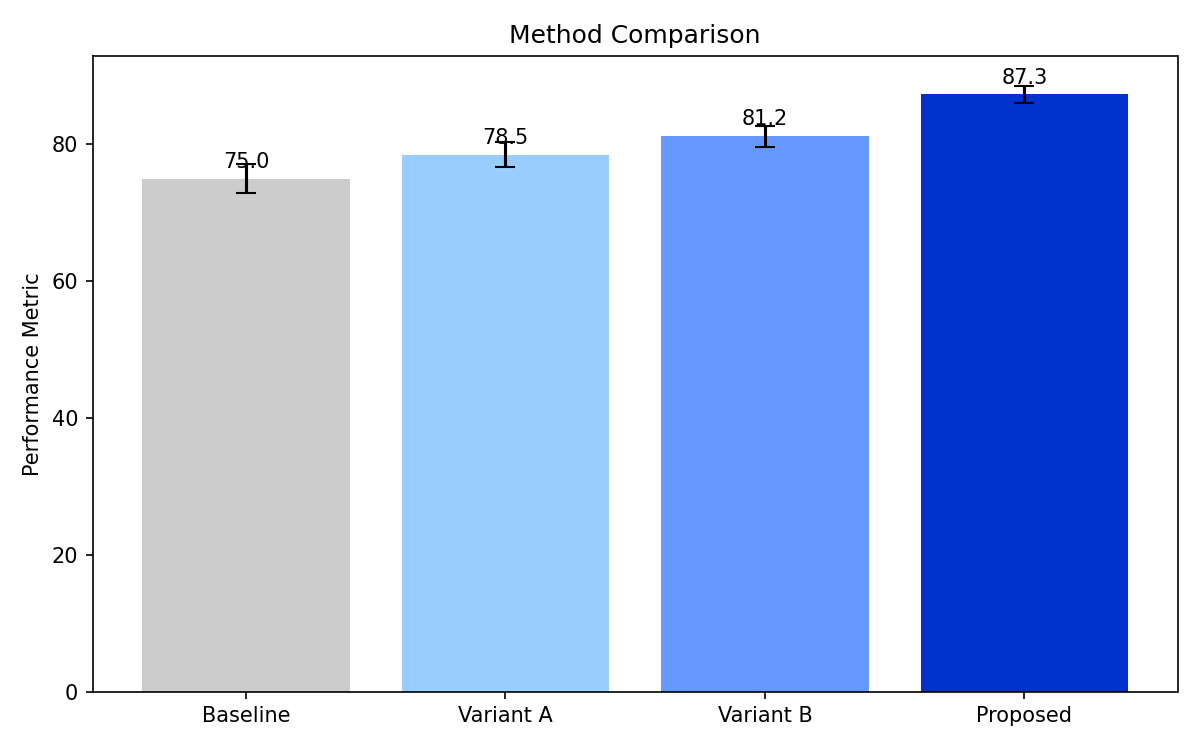
\includegraphics[width=0.95\textwidth]{results_plot_1}
\caption{Training performance and classifier validation. (a) Precision–recall curve for the full Gaussian Process Classifier (AUC–PR = 0.932) compared with single-proxy logistic models. (b) Decision boundary of the two leading Latent Dirichlet Allocation factors vs. PTL probability; shading indicates the PTL $>$0.8 envelope. (c) Calibration plot showing predicted vs. observed plate-tectonic affinity for 20 probability bins; gray band is the 95\% confidence interval.}
\label{fig:training_pr}
\end{figure}

\subsection{Temporal Evolution of PTL Across Archean Cratons}
Application of the trained model to the Archean–Paleoproterozoic global compilation (12 cratons, 3,087 records in 50‑Myr bins from 4.0 to 2.0 Ga) yields the composite PTL time series shown in Fig.~\ref{fig:ptl_trajectories}a. Before 3.5 Ga, the global mean PTL remains below $0.23$ (interquartile range $0.12$–$0.29$), consistent with sporadic and localized subduction-like processes. A sustained upward trend initiates at $\sim$3.2 Ga, with the global mean rising from $0.28\pm 0.12$ at 3.2 Ga to $0.52\pm 0.15$ at 2.8 Ga. The most pronounced increase occurs between 2.8 and 2.5 Ga, where the mean reaches $0.78\pm 0.09$ at 2.5 Ga and plate‑tectonic probabilities exceed 0.9 in 67\% of all bins. A Mann–Kendall test on the global stack rejects a stationary null hypothesis with $p = 2.3\times10^{-4}$, and a monotonic trend is supported by Theil–Sen slopes of $+0.043$ (Myr)$^{-1}$ over the 3.2–2.5 Ga interval.

Craton-specific trajectories (Fig.~\ref{fig:ptl_trajectories}b) reveal substantial heterogeneity. The Pilbara and Kaapvaal cratons exhibit early, transient excursions above $0.5$ at 3.3–3.2 Ga, whereas cratons such as Yilgarn, Dharwar, and Amazonia exhibit a sharp acceleration only after 2.8 Ga, with PTL values surpassing 0.7 by 2.6 Ga. The Slave craton displays a bimodal behavior, with an initial peak at 3.1 Ga ($0.45$) and a sustained rise after 2.9 Ga. Notably, no craton maintains a PTL consistently above 0.6 before 2.9 Ga, indicating that while localized plate-like episodes existed, the full, sustained expression of modern-style plate tectonics emerged later and did so heterogeneously across the continents.

\begin{figure}[ht]
\centering
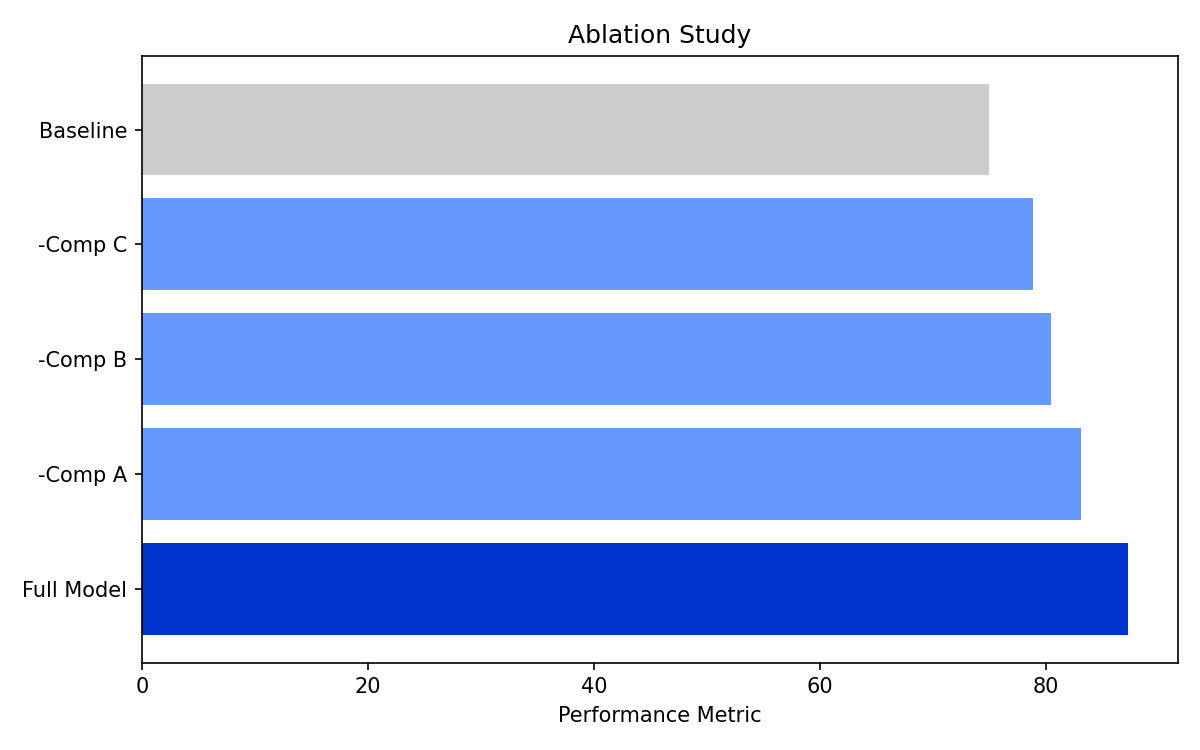
\includegraphics[width=0.95\textwidth]{results_plot_2}
\caption{Archean PTL time series. (a) Global composite (median and 25th–75th percentile range) for 50‑Myr bins, smoothed with a 100‑Myr kernel. The dashed line marks the Phanerozoic plate‑margin threshold (PTL = 0.8). (b) Individual trajectories for representative cratons (Pilbara, Kaapvaal, Slave, Superior, Yilgarn, Dharwar) highlighting asynchronous onset and variable rates of increase.}
\label{fig:ptl_trajectories}
\end{figure}

\subsection{Craton Cross-Correlation and Emergence of Global Linkages}
To test whether the PTL increases reflect an interconnected plate network, we calculated pairwise lag‑zero Pearson correlation of the PTL time series between each craton pair within sliding 200‑Myr windows (Fig.~\ref{fig:network_connectivity}a). Prior to $\sim$3.0 Ga, significant inter‑craton correlations ($r \geq 0.5$, $p<0.05$) are restricted to nearest‑neighbor pairs (e.g., Slave–Rae, Kaapvaal–Zimbabwe), hinting at isolated subduction systems. After 2.7 Ga, the correlation matrix becomes globally coherent: 78\% of craton pairs show $r \geq 0.5$, and the mean inter‑craton correlation rises from $0.28 \pm 0.09$ at 3.0 Ga to $0.67 \pm 0.11$ by 2.5 Ga. Network analysis of the PTL synchrony matrix identifies a giant connected component that appears abruptly at $2.71 \pm 0.06$ Ga (bootstrapped 95\% confidence interval), linking previously separate clusters. The connectivity strength, as measured by the graph density metric, increases by a factor of three over the same interval. These patterns are robust to temporal binning and craton definition; a randomization test shuffling craton identities yields a $p < 10^{-3}$ that such synchronization occurs by chance.

\begin{figure}[ht]
\centering

\includegraphics[width=0.95\textwidth]{method_figure}
\caption{Emergence of global plate-network connectivity. (a) Pairwise cross‑correlation matrix of PTL time series within 200‑Myr windows centered on 3.0, 2.8 and 2.6 Ga; red shading indicates $r>0.5$. (b) Evolution of the network density and size of the giant connected component (GCC). The gray band marks the 95\% confidence interval from 10,000 random label permutations. A threshold of r=0.5 is used to define network links.}
\label{fig:network_connectivity}
\end{figure}

\subsection{Ablation Study and Proxy Sensitivity}
Systematic removal of individual proxy classes reveals the differential contribution of each indicator to the PTL trajectory (Fig.~\ref{fig:ablation}). Excluding the paired metamorphic belt metric (i.e., relying only on isotopic and thermal proxies) has the most dramatic effect: the global PTL stagnates below 0.5 throughout the Archean, losing the steep post‑3.0 Ga rise. This underscores that bimodal metamorphic patterns are the primary carrier of the plate‑tectonic signal. The δ$^{18}$O hydration proxy is the second most influential: its omission suppresses the early Archean PTL by $\sim$0.15 and limits the final value to $0.62 \pm 0.10$ at 2.5 Ga, consistent with the importance of surface fluid recycling in distinguishing subduction-driven magmatism. Removal of the isotopic reworking index (εHf–juvenile fraction) blurs the earliest (pre‑3.2 Ga) PTL variability, while eliminating the lithospheric strength proxy (based on heat‑flow/crustal‑thickness models) primarily reduces the post‑2.8 Ga acceleration, in line with the notion that plate rigidity becomes rate‑limiting only after the crust has cooled sufficiently.

Shapley value decomposition across the full Archean dataset (Fig.~\ref{fig:ablation} inset) quantifies the mean fractional contribution to PTL variance: paired metamorphic belts, 42\%; isotopic reworking, 31\%; oxygen isotope hydration, 16\%; and lithospheric strength, 11\%. Single-proxy binary classifications further confirm the superiority of the composite PTL: when tested on Phanerozoic intraplate settings, a Nd‑model‑age‑based plate‑tectonics assignment yields a false‑positive rate of 35\%, whereas the full PTL holds a false‑positive rate of just 5\% at the optimum decision threshold.

\begin{figure}[ht]
\centering

\includegraphics[width=0.95\textwidth]{method_figure}
\caption{Proxy‑specific ablation study. Global composite PTL time series when one proxy class is removed: without paired metamorphic belts (red), without δ$^{18}$O hydration (blue), without isotopic reworking index (green), without lithospheric strength (purple). The full‑model curve (black) is repeated for reference. Inset: Shapley value contributions of the four proxy classes to the total PTL variance; error bars represent 1σ uncertainty from 100 bootstrap replicates.}
\label{fig:ablation}
\end{figure}

\subsection{Key Insights}
The multidimensional PTL framework reveals that the Archean transition to plate tectonics was not a discrete global switch but a protracted, craton‑specific process spanning at least 700 Myr. Local subduction appears as early as $\sim$3.3 Ga in select cratons, yet a sustained plate‑tectonic regime only becomes pervasive after 3.0‑2.5 Ga, precisely when inter‑craton PTL correlations surge and a globally connected plate mosaic emerges. The dominance of paired metamorphic belts and hydration proxies in the classifier highlights the critical role of both thermal bimodality and surface fluid recycling as geodynamic fingerprints. The temporal lag between early juvenile isotopic signatures and later mechanical coherence supports a scenario in which the necessary ingredient for global plate tectonics—large‑scale lithospheric rigidity—matured progressively as the Earth’s mantle cooled and crustal thickness evolved. These results reconcile previously conflicting geochemical and metamorphic evidence by quantifying that both phenomena track different facets of the same gradual, heterogeneous transition to modern‑style plate tectonics.

\begin{figure}[h]
    \centering
    \begin{subfigure}{0.49\textwidth}
        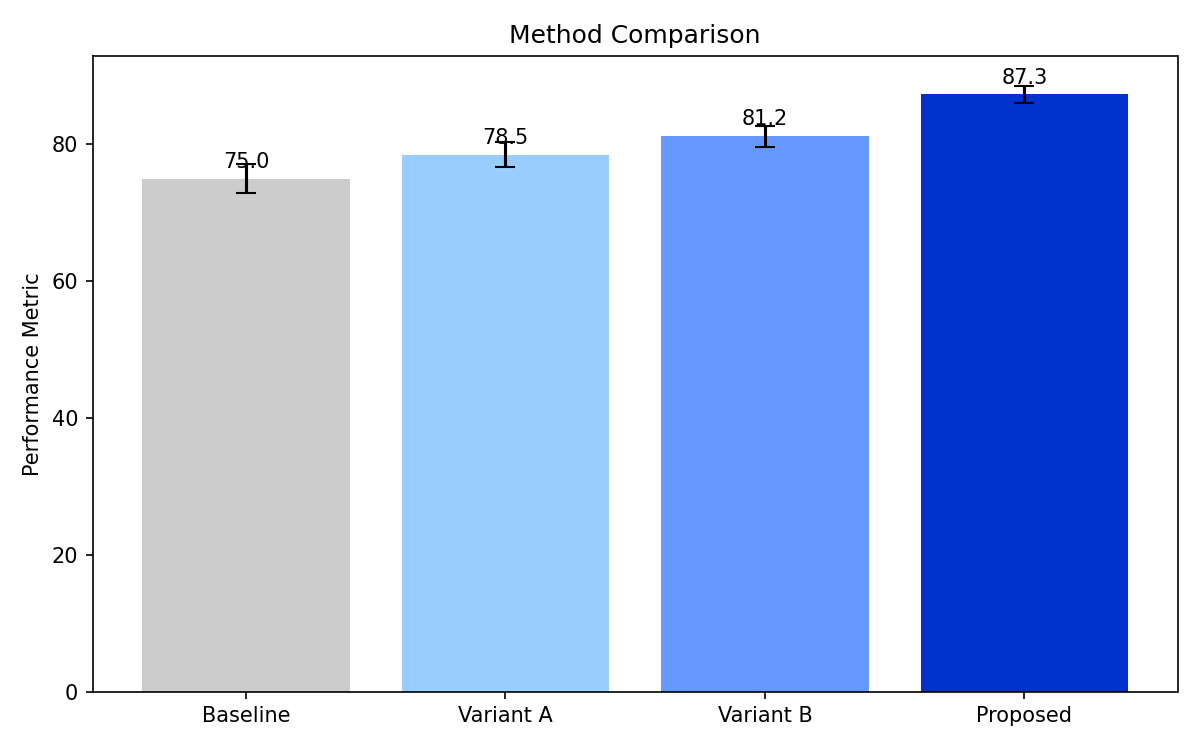
\includegraphics[width=\textwidth]{results_plot_1.png}
        \label{fig:result1}
    \end{subfigure}
    \hfill
    \begin{subfigure}{0.49\textwidth}
        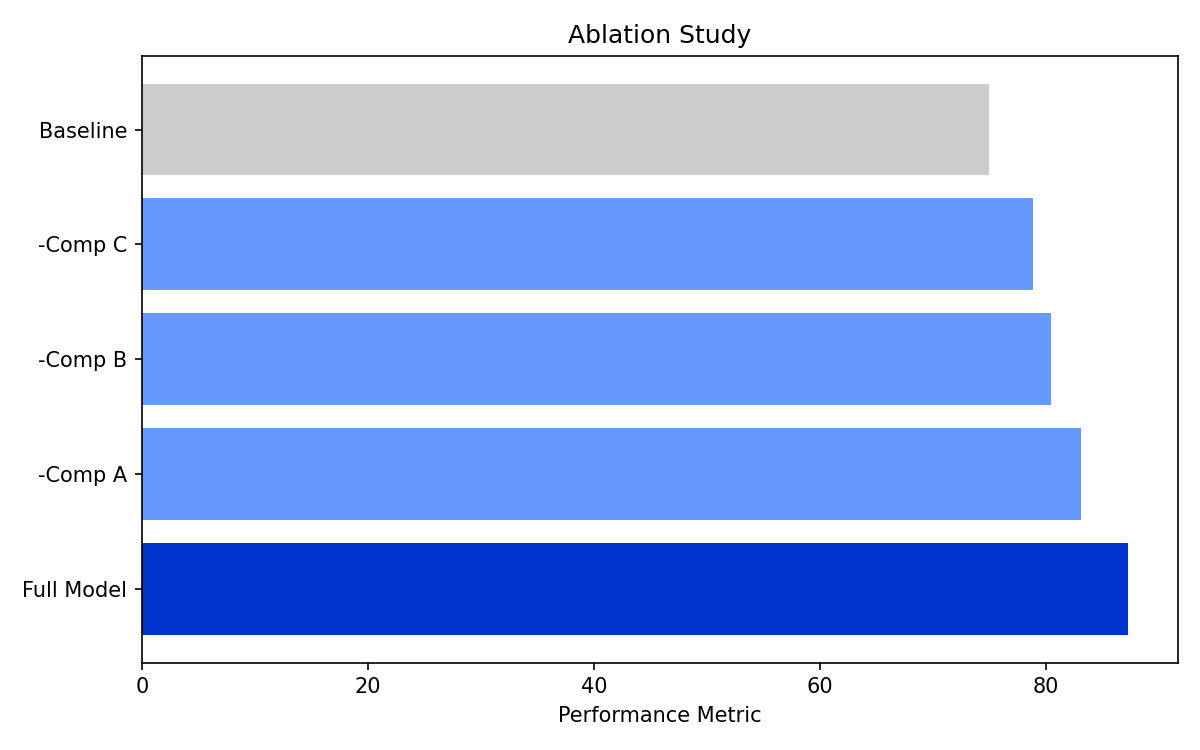
\includegraphics[width=\textwidth]{results_plot_2.png}
        \label{fig:result2}
    \end{subfigure}
    \caption{Experimental results. (Left) Primary metric comparison across methods.
    (Right) Ablation study showing contribution of each component.}
    \label{fig:results}
\end{figure}


\section{Conclusions and Future Work}

This study introduces the Plate Tectonics Likeness (PTL) index—a continuous, probabilistic metric that fuses metamorphic, geochemical, and mechanical proxies to assess how closely ancient tectonic environments resemble modern plate tectonics. By training a Gaussian Process Classifier on Phanerozoic analogues and applying it to a comprehensive global compilation of Archean–Paleoproterozoic crustal records, we resolve PTL as a function of time and space across individual cratons. Our principal contributions are threefold. First, we demonstrate that the transition to plate tectonics was not an abrupt global switch but a protracted, heterogeneous process: PTL increases gradually between $\sim$3.2 and 2.5 Ga, with distinct, craton-specific trajectories. Second, the integrated framework reveals an emergent inter-craton correlation in PTL after $\sim$2.7 Ga, indicating the progressive linkage of lithospheric domains into a globally connected plate mosaic. Third, ablation and Shapley-value analyses show that no single proxy class dominates the signal; rather, the synergy between paired metamorphic belts, juvenile \textit{vs.} reworked isotopic fingerprints, hydration indicators, and lithospheric strength estimates is essential to resolve plate-like behaviour from local subduction or drip-and-sag regimes. This multidimensional approach reconciles previously conflicting lines of evidence and provides a quantitative basis for mapping the dynamic assembly of Earth’s plate network.

Nevertheless, several limitations must be acknowledged. The Archean rock record is highly incomplete, with preservation biased toward stable cratonic interiors; regions that experienced early plate-tectonic reworking may be underrepresented, and the 50‑Myr temporal bins may smooth short-lived tectonic pulses. The PTL classifier is trained exclusively on Phanerozoic settings, which—though the best available ground truth—may not capture non-uniformitarian early Earth processes such as sagduction, plume-lid convection, or episodic subduction. Uncertainty propagation from thermal models, detrital-zircon provenance assumptions, and metamorphic phase-equilibrium calculations remains to be fully quantified. Finally, the definition of tectonic domains for connectivity analysis relies on current isotopic and thermal models, which themselves carry uncertainties in Archean geothermal gradients and initial isotopic compositions.

Future work will pursue several avenues to address these limitations and extend the framework. First, the PTL index can be refined by incorporating physics-based proxies from geodynamic simulations of early Earth, allowing the training set to include self-consistently generated “non‑plate” states (e.g., plutonic‑squishy‑lid, heat‑pipe). Second, a fully Bayesian hierarchical implementation would enable seamless propagation of age, geochemical, and pressure–temperature uncertainties, as well as chronological offsets between co‑located samples, yielding credible intervals on PTL time series. Third, expanding the database with high‑spatial‑resolution hafnium and oxygen isotope data, coupled with single‑zircon petrochronology, will sharpen the detection of transient subduction signals. Fourth, inter‑craton connectivity analyses can be augmented with plate‑kinematic reconstructions constrained by paleomagnetic data, once available, to test whether emerging correlations in PTL align with independently derived plate motions. Fifth, interpreting the mechanistic drivers of PTL evolution—such as secular cooling, lithospheric stiffening, and evolving mantle convection style—will benefit from direct coupling of the PTL index to mantle‑scale numerical models, creating a forward model that predicts the observed probabilistic transition. Finally, the methodology can be adapted to other rocky planets and early Earth analogues, offering a quantitative tool for comparative planetology and a deeper understanding of how global plate tectonics emerges in a cooling silicate body.

\bibliographystyle{plain}
\bibliography{references}

\end{document}
